\documentclass{scrreprt}

\usepackage{aligned-overset}
\usepackage{amsmath}
\usepackage{amsthm}
\usepackage{amssymb}
\usepackage{bm}
\usepackage[inline,shortlabels]{enumitem}
\usepackage{framed}
\usepackage{hyperref}
\usepackage[utf8]{inputenc}
\usepackage{multicol}
\usepackage{mathtools}
\usepackage{pdflscape}
\usepackage{physics}
\usepackage{polynom}
\usepackage{tabularx}
\usepackage[table]{xcolor}
\usepackage{titling}
\usepackage{fancyhdr}
\usepackage{xfrac}
\usepackage{pgfplots}

\pgfplotsset{compat = newest}
\usepgfplotslibrary{fillbetween}
\usetikzlibrary{calc}


\author{Karsten Lehmann}
\date{WiSe 2024/25}
\title{Übungsblatt 12\\INF-B-110, Lineare Algebra}

\setlength{\parindent}{0pt}

\setlength{\headheight}{26pt}
\pagestyle{fancy}
\fancyhf{}
\lhead{\thetitle}
\rhead{\theauthor}
\lfoot{\thedate}
\rfoot{Seite \thepage}

\begin{document}
\paragraph{Ü 12.3 über Matrizen definierte Skalarprodukte}

Betrachtet wird die Abbildung
$s \colon \mathbb{R}^2 \times \mathbb{R}^2 \to \mathbb{R},
\qty\big{u, v} \mapsto u^T \begin{pmatrix}
  3 & 1 \\
  1 & 3 \\
\end{pmatrix} v$.
\begin{enumerate}[(a)]
\item Zeigen Sie, dass $s$ ein Skalarprodukt auf $\mathbb{R}^2$ ist

  \subparagraph{Lsg.} Sei $M = \begin{pmatrix}
    3 & 1 \\
    1 & 3 \\
  \end{pmatrix}$,
  Es ist zu zeigen, dass $s$ folgende Eigenschaften
  besitzt:
  \begin{enumerate}[(1)]
  \item \textbf{Bilinearität:} Es ist
    \begin{flalign*}
      \qty\big(u_1 + u_2) \bullet v &= \qty\big(u_1 + u_2)^TMv \\
      \overset{\text{Distributivität}}&= u_1^TMv + u_2^TMv \\
      &= u_1 \bullet v + u_2 \bullet v
    \end{flalign*}
    sowie
    \begin{flalign*}
      u + \qty\big(v_1 + v_2) \bullet v &= u^TM\qty\big(v_1 + v_2) \\
      \overset{\text{Distributivität}}&= u^TMv_1 + u^TMv_2 \\
      &= u \bullet v_1 + u \bullet v_2
    \end{flalign*}
    und
    \begin{flalign*}
      \qty\big(\lambda \cdot u) \bullet \qty\big(\mu \cdot v)
      &= \qty\big(\lambda \cdot u)^TM\qty\big(\mu \cdot v) \\
      &= \lambda\mu u^TMv \\
      &= \lambda\mu\qty\big(u \bullet v)
    \end{flalign*}

  \item \textbf{Symmetrie:} Es ist
    \[
      u \bullet v \overset{\text{Transponierung egal weil Skalar}}=
      \qty\big(u \bullet v)^T = \qty\big(u^TMv^T)
      = v^TM^Tu
      \overset{M \text{ ist symmetrisch}}= v^TMu
    \]

  \item \textbf{Positive Definitheit:} Sei
    $u = \begin{pmatrix} x \\ y \end{pmatrix} \in \mathbb{R}^2$.
    Dann ist
    \begin{flalign*}
      u \bullet u &= \qty\big(x, y) \begin{pmatrix}
        3 & 1 \\
        1 & 3 \\
      \end{pmatrix} \begin{pmatrix}
        x \\
        y \\
      \end{pmatrix} \\
      &= \qty\big(3x + y, x + 3y) \begin{pmatrix}
        x \\
        y \\
      \end{pmatrix} \\
      &= 3x^2 + 2xy + 3y^2 \\
      &= 2x^2 + x^2 + 2xy + y^2 + 2y^2 \\
      &= \underset{\geq 0}{\underbrace{2x^2}} + \underset{\geq 0}{\underbrace{\qty\big(x + y)^2}} + \underset{\geq 0}{\underbrace{2y^2}}
    \end{flalign*}
    Außerdem ist offensichtlich, dass $u \bullet u = 0 \iff x = y = 0$.
  \end{enumerate}

\newpage
\item Berechnen Sie die Norm der Vektoren $v_1 = \qty\big(1, 1)^T$ und
  $v_2 = \qty\big(-2, 2)^T$ bezüglich $s$.
  Sind $v_1$ und $v_2$ orthogonal bezüglich $s$?

  \subparagraph{Lsg.} Es sind
  \begin{flalign*}
    \norm{\begin{pmatrix}
      1 \\
      1 \\
    \end{pmatrix}} &= \sqrt{
      \begin{pmatrix}
        1 \\
        1 \\
      \end{pmatrix}
      \bullet
      \begin{pmatrix}
        1 \\
        1 \\
      \end{pmatrix}
    } \\
    &= \sqrt{
      \qty\big(1, 1) \begin{pmatrix}
        3 & 1 \\
        1 & 3 \\
      \end{pmatrix} \begin{pmatrix}
        1 \\
        1\\
      \end{pmatrix}
    } \\
    &= \sqrt{
      \qty\big(4, 4) \begin{pmatrix}
        1 \\
        1 \\
      \end{pmatrix}
    } \\
    &= \sqrt{8}
  \end{flalign*}
  sowie
  \begin{flalign*}
    \norm{\begin{pmatrix}
      -2 \\
      2  \\
    \end{pmatrix}} &= \sqrt{
      \begin{pmatrix}
        -2 \\
        2  \\
      \end{pmatrix}
      \bullet
      \begin{pmatrix}
        -2 \\
        2  \\
      \end{pmatrix}
    } \\
    &= \sqrt{
      \qty\big(-2, 2) \begin{pmatrix}
        3 & 1 \\
        1 & 3 \\
      \end{pmatrix} \begin{pmatrix}
        -2 \\
        2  \\
      \end{pmatrix}
    } \\
    &= \sqrt{
      \qty\big(-4, 4) \begin{pmatrix}
        -2 \\
        2  \\
      \end{pmatrix}
    } \\
    &= \sqrt{16} = 4
  \end{flalign*}
  und schließlich
  \[
    \begin{pmatrix}
      1 \\
      1 \\
    \end{pmatrix}
    \bullet
    \begin{pmatrix}
      -2 \\
      2  \\
    \end{pmatrix}
    =
    \qty\big(1, 1) \begin{pmatrix}
      3 & 1 \\
      1 & 3 \\
    \end{pmatrix} \begin{pmatrix}
      -2 \\
      2  \\
    \end{pmatrix}
    =
    \qty\big(4, 4) \begin{pmatrix}
      -2 \\
      2  \\
    \end{pmatrix}
    = 0
  \]
  Somit sind die beiden Vektoren orthogonal zueinander.
\end{enumerate}

\newpage
\paragraph{Ü 12.4 Längen und Normen}

Sei $V = \mathbb{R}^2$ und $\bullet$ das Standardskalarprodukt.
Bestimmen Sie alle Einheitsvektoren $v \in \mathbb{R}^2$, die von
$u = \qty\big(1, 1)^T$ den Abstand $\sqrt{2}$ haben.
Fertigen Sie eine passende Skizze an.

\subparagraph{Lsg.} Die Skizze:

\begin{tikzpicture}
  \begin{axis}[
    axis equal image,
    axis x line=center,
    axis y line=center,
    grid=both,
    xmin=-1.5,
    xmax=1.5,
    xtick distance=1,
    ymin=-1.5,
    ymax=1.5,
    ytick distance=1,
  ]
    \node[circle, draw, inner sep=0pt, minimum size=1mm,label=above:{$u$}] (1) at (1,1) {};
    \node[circle, draw, inner sep=0pt, minimum size=1mm,label=above:{$v_1$}] (2) at ($(-{(sqrt(7) - 1)/4},{(1 + sqrt(7))/4})$) {};
    \node[circle, draw, inner sep=0pt, minimum size=1mm,label=left:{$v_2$}] (3) at ($({(sqrt(7) + 1)/4},{(1 - sqrt(7))/4})$) {};
    \addplot[domain=-1:1, name path=A, smooth] { sqrt(1 - \x^2)};
    \addplot[domain=-1:1, name path=B, smooth] { -sqrt(1 - \x^2)};

    \draw[dashed, ->] (1) -- (2) node[midway, label=above:{$\sqrt{2}$}] {};
    \draw[dashed, ->] (1) -- (3) node[midway, label=right:{$\sqrt{2}$}] {};
  \end{axis}

\end{tikzpicture}

Nun ist
\begin{flalign*}
  \norm{v} &= 1 \\
  \sqrt{v_1^2 + v_2^2} &= 1 && {\Big |} \qty\big(\ldots)^2 &&&& \\
  v_1^2 + v_2^2 &= 1
\end{flalign*}
und
\begin{flalign*}
  \norm{u - v} &= \sqrt{2} \\
  \sqrt{\qty\big(1 - v_1)^2 + \qty\big(1 - v_2)^2} &= \sqrt{2} && {\Big |} \qty\big(\ldots)^2 &&&& \\
  \qty\big(1 - v_1)^2 + \qty\big(1 - v_2)^2 &= 2 \\
  2 - 2v_1 - 2 v_2 + v_1^2 + v_2^2 &= 2 && {\Big |} \text{siehe erste Gleichung} \\
  2 - 2v_1 - 2 v_2 &= 1 \\
  v_1 = \frac{1 - 2v_2}{2}
\end{flalign*}
Jetzt setzt man $v_1$ wieder in die erste Gleichung ein und erhält
\begin{flalign*}
  \frac{1 - 2v_2}{2}^2 + v_2^2 &= 1 \\
  \frac{\qty\big(1 - 2v_2)^2}{4} + v_2^2 &= 1 \\
  \frac{1 - 4v_2 + 4v_2^2}{4} + v_2^2 &= 1 \\
  \frac{1}{4} - v_2 + 2v_2^2 &= 1 \\
  v_2^2 - \frac{v_2}{2} - \frac{3}{8} &= 0
\end{flalign*}
Und mit der $p$-$q$-Formel:
\begin{flalign*}
  v_2 &= \frac{1}{4} \pm \sqrt{\frac{1}{16} + \frac{6}{16}} \\
      &= \frac{1}{4} \pm \frac{\sqrt{7}}{4}
\end{flalign*}
Setzt man dies wieder in die erste Gleichung ein, dann folgen die beiden Vektoren
\begin{flalign*}
  \begin{pmatrix}
    -\frac{1}{4}\qty\big(\sqrt{7} - 1) \\
    \frac{1 + \sqrt{7}}{4} \\
  \end{pmatrix} \text{ und } \begin{pmatrix}
    \frac{1}{4}\qty\big(\sqrt{7} + 1) \\
    \frac{1 - \sqrt{7}}{4} \\
  \end{pmatrix}
\end{flalign*}

\paragraph{Ü 12.5 Beweise mit Hilfe der Eigenschaften des Skalarproduktes}

Es sei $V$ ein Euklidischer Vektorraum mit Skalarprodukt $s$ und der dadurch
induzierten Norm $\norm{\cdot}\colon V \to \mathbb{R},
v \mapsto \sqrt{v \bullet v}$.
Zeigen Sie die
\[
  \emph{Parallelogrammgleichung}: \forall x, y \in V \colon
  \norm{x + y}^2 + \norm{x - y}^2 = 2\norm{x}^2 + 2 \norm{y}^2
  \text{ und die}
\]
\[
  \emph{Polarisierungsidentität}: \forall x, y \in V \colon
  x \bullet y = \frac{1}{4}\qty(\norm{x + y}^2 - \norm{x - y}^2)
\]

\subparagraph{Lsg.} Es ist
\begin{flalign*}
  \norm{x + y}^2 + \norm{x - y}^2
  &= \sqrt{\qty\big(x + y) \bullet \qty\big(x + y)}^2 + \sqrt{\qty\big(x - y) \bullet \qty\big(x - y)}^2 \\
  &= \qty\big(x + y) \bullet \qty\big(x + y) + \qty\big(x - y) \bullet \qty\big(x - y) \\
  \overset{\text{bilinear}}&= x \bullet \qty\big(x + y) + y \bullet \qty\big(x + y) + x \bullet \qty\big(x - y) - y \bullet \qty\big(x - y) \\
  \overset{\text{bilinear}}&= x \bullet x + x \bullet y + y \bullet x + y \bullet y + x \bullet x -  x \bullet y - y \bullet x + y \bullet y \\
  &= 2 \cdot \qty\big(x \bullet x) + 2 \cdot \qty\big(y \bullet y) \\
  &= 2 \cdot \sqrt{\qty\big(x \bullet x)}^2 + 2 \cdot \sqrt{\qty\big(y \bullet y)}^2 \\
  &= 2 \cdot \norm{x}^2 + 2\norm{y}^2
\end{flalign*}
\newpage
Und
\begin{flalign*}
  \frac{1}{4}\qty(\norm{x + y}^2 - \norm{x - y}^2)
  &= \frac{1}{4}\qty(\sqrt{\qty\big(x + y) \bullet \qty\big(x + y)}^2 - \sqrt{\qty\big(x - y) \bullet \qty\big(x - y)}^2) \\
  &= \frac{1}{4}\qty(\qty\big(x + y) \bullet \qty\big(x + y) - \qty\big(x - y) \bullet \qty\big(x - y)) \\
  \overset{\text{bilinear}}&= \frac{1}{4}\qty(x \bullet x + x \bullet y + y \bullet x + y \bullet y - x \bullet x + x \bullet y + y \bullet x - y \bullet y) \\
  &= \frac{1}{4}\qty(2\qty\big(x \bullet y) + 2\qty\big(y \bullet x)) \\
  \overset{\text{Symmetrie}}&= \frac{1}{4}\qty(4\qty\big(x \bullet y)) \\
  &= x \bullet y
\end{flalign*}

\newpage
\paragraph{Ü 12.6 Orthogonalität und Orthogonalraum}

Bestimmen Sie zwei Vektoren $w_1, w_2 \in \mathbb{R}^4$, deren Norm 1 beträgt
und die zu den Vektoren $v_1 = \qty\big(2, 1, -4, 0)^T$,
$v_2 = \qty\big(-1, -1, 2, 2)^T$ sowie $v_3 = \qty\big(3, 2, 5, 4)^T$
(bzgl. des Standardskalarproduktes) orthogonal sind.

Berechnen Sie zum Untervektorraum $U = \text{Span}\qty\big{v_1, v_2, v_3}$ den
Orthogonalraum $U^{\bot} \subseteq \mathbb{R}^4$.

\subparagraph{Lsg.} Ein Vektor $u = \qty\big(a, b, c, d) \in \mathbb{R}^4$ ist
orthogonal zu $v_1$ genau dann wenn
\[
  2 \cdot a + 1 \cdot b - 4 \cdot c + 0 \cdot d = 0
\]
Analog zu den beiden anderen Vektoren.
Dementsprechend ist der Orthogonalraum
\begin{flalign*}
  U^{bot} &= \text{Ker}\begin{pmatrix}
    2  & 1  & -4 & 0 \\
    -1 & -1 & 2  & 2 \\
    3  & 2  & 5  & 4 \\
  \end{pmatrix} \\
  \overset{Z_3 = Z_3 + 3 \cdot Z_2}&= \text{Ker}\begin{pmatrix}
    2  & 1  & -4 & 0  \\
    -1 & -1 & 2  & 2  \\
    0  & -1 & 11 & 10 \\
  \end{pmatrix} \\
  \overset{Z_2 = 2 \cdot Z_2 + Z_1}&= \text{Ker}\begin{pmatrix}
    2 & 1  & -4 & 0  \\
    0 & -1 & 0  & 4  \\
    0 & -1 & 11 & 10 \\
  \end{pmatrix} \\
  \overset{Z_3 = Z_3 - Z_2}&= \text{Ker}\begin{pmatrix}
    2 & 1  & -4 & 0 \\
    0 & -1 & 0  & 4 \\
    0 & 0  & 11 & 6 \\
  \end{pmatrix} \\
  \overset{Z_1 = \frac{1}{2}\qty\big(Z_1 + Z_2)}&= \text{Ker}\begin{pmatrix}
    1 & 0  & -2 & 2 \\
    0 & -1 & 0  & 4 \\
    0 & 0  & 11 & 6 \\
  \end{pmatrix} \\
  \overset{Z_1 = Z_1 + \frac{2}{11} \cdot Z_3}&= \text{Ker}\begin{pmatrix}
    1 & 0  & 0  & \frac{34}{11} \\
    0 & -1 & 0  & 4             \\
    0 & 0  & 11 & 6             \\
  \end{pmatrix} \\
  &= \qty{
    \begin{pmatrix}
      -\frac{34}{11}x_4 \\
      4x_4              \\
      \frac{6}{11}x_4   \\
      x_4               \\
    \end{pmatrix}
    \:\middle|\:
    x_4 \in \mathbb{R}
  } \\
  &= \text{Span}\qty{
    \begin{pmatrix}
      -34 \\
      44  \\
      6   \\
      11  \\
    \end{pmatrix}
  }
\end{flalign*}
Nun ist die Norm der Basis des Orthogonalraums
\[
  \norm{b} =
  \norm{
    \begin{pmatrix}
      -34 \\
      44  \\
      -6  \\
      11  \\
    \end{pmatrix}
  } = \sqrt{\qty\big(-34)^2 + 44^2 + \qty\big(-6)^2 + 11^2} = 57
\]
und
\[
  w_1 = \frac{b}{\norm{b}} = \frac{1}{57} \begin{pmatrix}
    -34 \\
    44  \\
    -6  \\
    11  \\
  \end{pmatrix} \text{ und } w_2 = -\frac{b}{\norm{b}} = -\frac{1}{57} \begin{pmatrix}
    -34 \\
    44  \\
    -6  \\
    11  \\
  \end{pmatrix}
\]

\end{document}
